% aRES quick report -- one-page poster-style summary.
% Build:  latexmk -pdf quick_report.tex
%
% Three figures are placeholders. Export each from PyMOL into figs/ under the
% name shown in its box, then replace the whole \figbox{...}{...}{...} call with
%     \includegraphics[width=\linewidth]{figs/<name>.png}

\documentclass[10pt,a4paper]{article}

\usepackage[T1]{fontenc}
\usepackage[utf8]{inputenc}
\usepackage[margin=1.15cm]{geometry}
\usepackage{graphicx}
\usepackage{booktabs}
\usepackage{xcolor}
\usepackage{enumitem}

\definecolor{zn}{HTML}{7B3F9D}
\definecolor{soft}{HTML}{777777}

\setlength{\parindent}{0pt}
\setlength{\parskip}{3pt}
\pagestyle{empty}

\newcommand{\panelhead}[1]{\par\vspace{1pt}{\LARGE #1}\par\vspace{3pt}}
\newcommand{\colhead}[1]{\par{\Large #1}\par\vspace{2pt}}
\newcommand{\divider}{\par\vspace{4pt}\noindent\rule{\linewidth}{1.1pt}\par\vspace{2pt}}

% Placeholder for a render that does not exist yet.
% #1 = height, #2 = target filename in figs/, #3 = what to render
\newcommand{\figbox}[3]{%
  \setlength{\fboxsep}{6pt}%
  \fbox{\begin{minipage}[c][#1][c]{\dimexpr\linewidth-2\fboxsep-2\fboxrule\relax}
    \centering\footnotesize\color{soft}%
    \texttt{\detokenize{figs/#2}}\par\vspace{4pt}#3\par
  \end{minipage}}}

\begin{document}

{\Huge Quick Report: initial findings on aRES}\par\vspace{1pt}
{\small\textcolor{soft}{\emph{E.~coli} UC5 aRES, 459 aa. Sequence composition and AlphaFold3 model
analysis only. No experimental data. \today}}

\vspace{5pt}

% ===================== ROW 1 =====================
\begin{minipage}[t]{0.48\linewidth}
\vspace{0pt}
\centerline{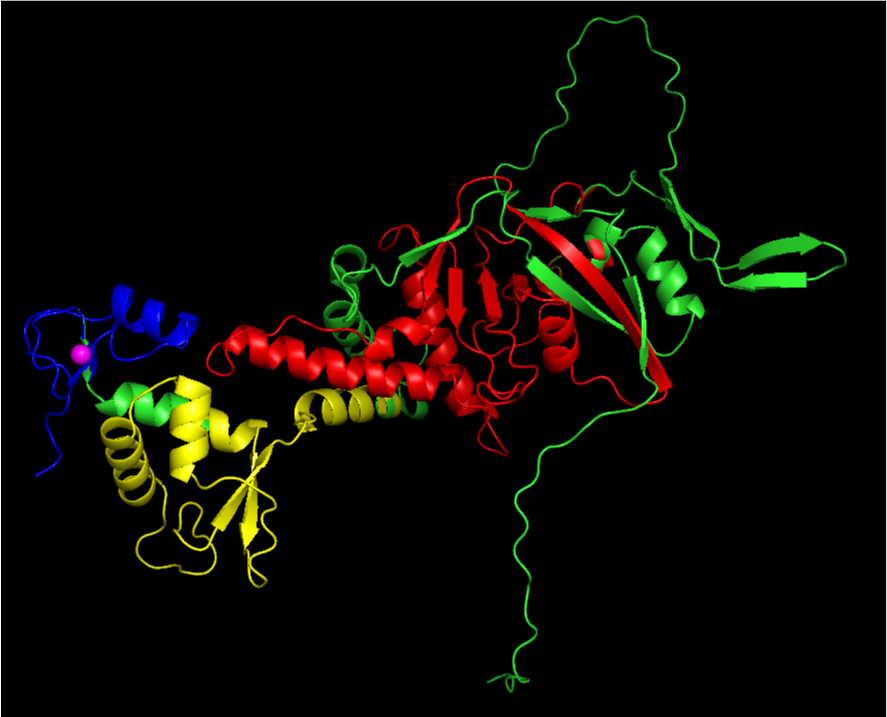
\includegraphics[height=5.8cm]{figs/nblock_cartoon.png}}
\vspace{2pt}
{\footnotesize Zn ribbon 1--48 blue, NTD-1 49--120 yellow, RES 126--447 red.}
\end{minipage}
\hfill
\begin{minipage}[t]{0.49\linewidth}
\vspace{0pt}
{\small Charge composition, Lys$+$Arg against Asp$+$Glu:}\par\vspace{3pt}
{\footnotesize
\begin{tabular}{@{}lrrrrrr@{}}
\toprule
Region & Len & K & R & D & E & Net (/100) \\
\midrule
Zn ribbon 1--48   &  48 & 10 &  3 &  2 &  0 & $\mathbf{+11}$ \ ($+22.9$) \\
NTD-1 49--120     &  72 &  0 &  3 & 11 &  8 & $\mathbf{-16}$ \ ($-22.2$) \\
N-block 1--120    & 120 & 10 &  6 & 13 &  8 & $-5$ \ ($-4.2$) \\
RES side 126--447 & 322 & 23 & 19 & 24 & 21 & $-3$ \ ($-0.9$) \\
\bottomrule
\end{tabular}}

\vspace{5pt}
{\small The two N-terminal modules carry equal and opposite charge density. The ribbon has ten
lysines and no glutamate. NTD-1 has nineteen acidic residues and no lysine. The RES domain is at
$-0.9$ per 100, so the extremity is confined to the N-block.

\vspace{3pt}
Residues 31--40 are \texttt{CSYC \textbf{KRKRK} N}, a basic run directly after the second CxxC.}
\end{minipage}

\divider

% ===================== ROW 2 =====================
\panelhead{Two N-terminal domains}

\begin{minipage}[t]{0.47\linewidth}
\vspace{0pt}
\colhead{1.\ NTD-1}
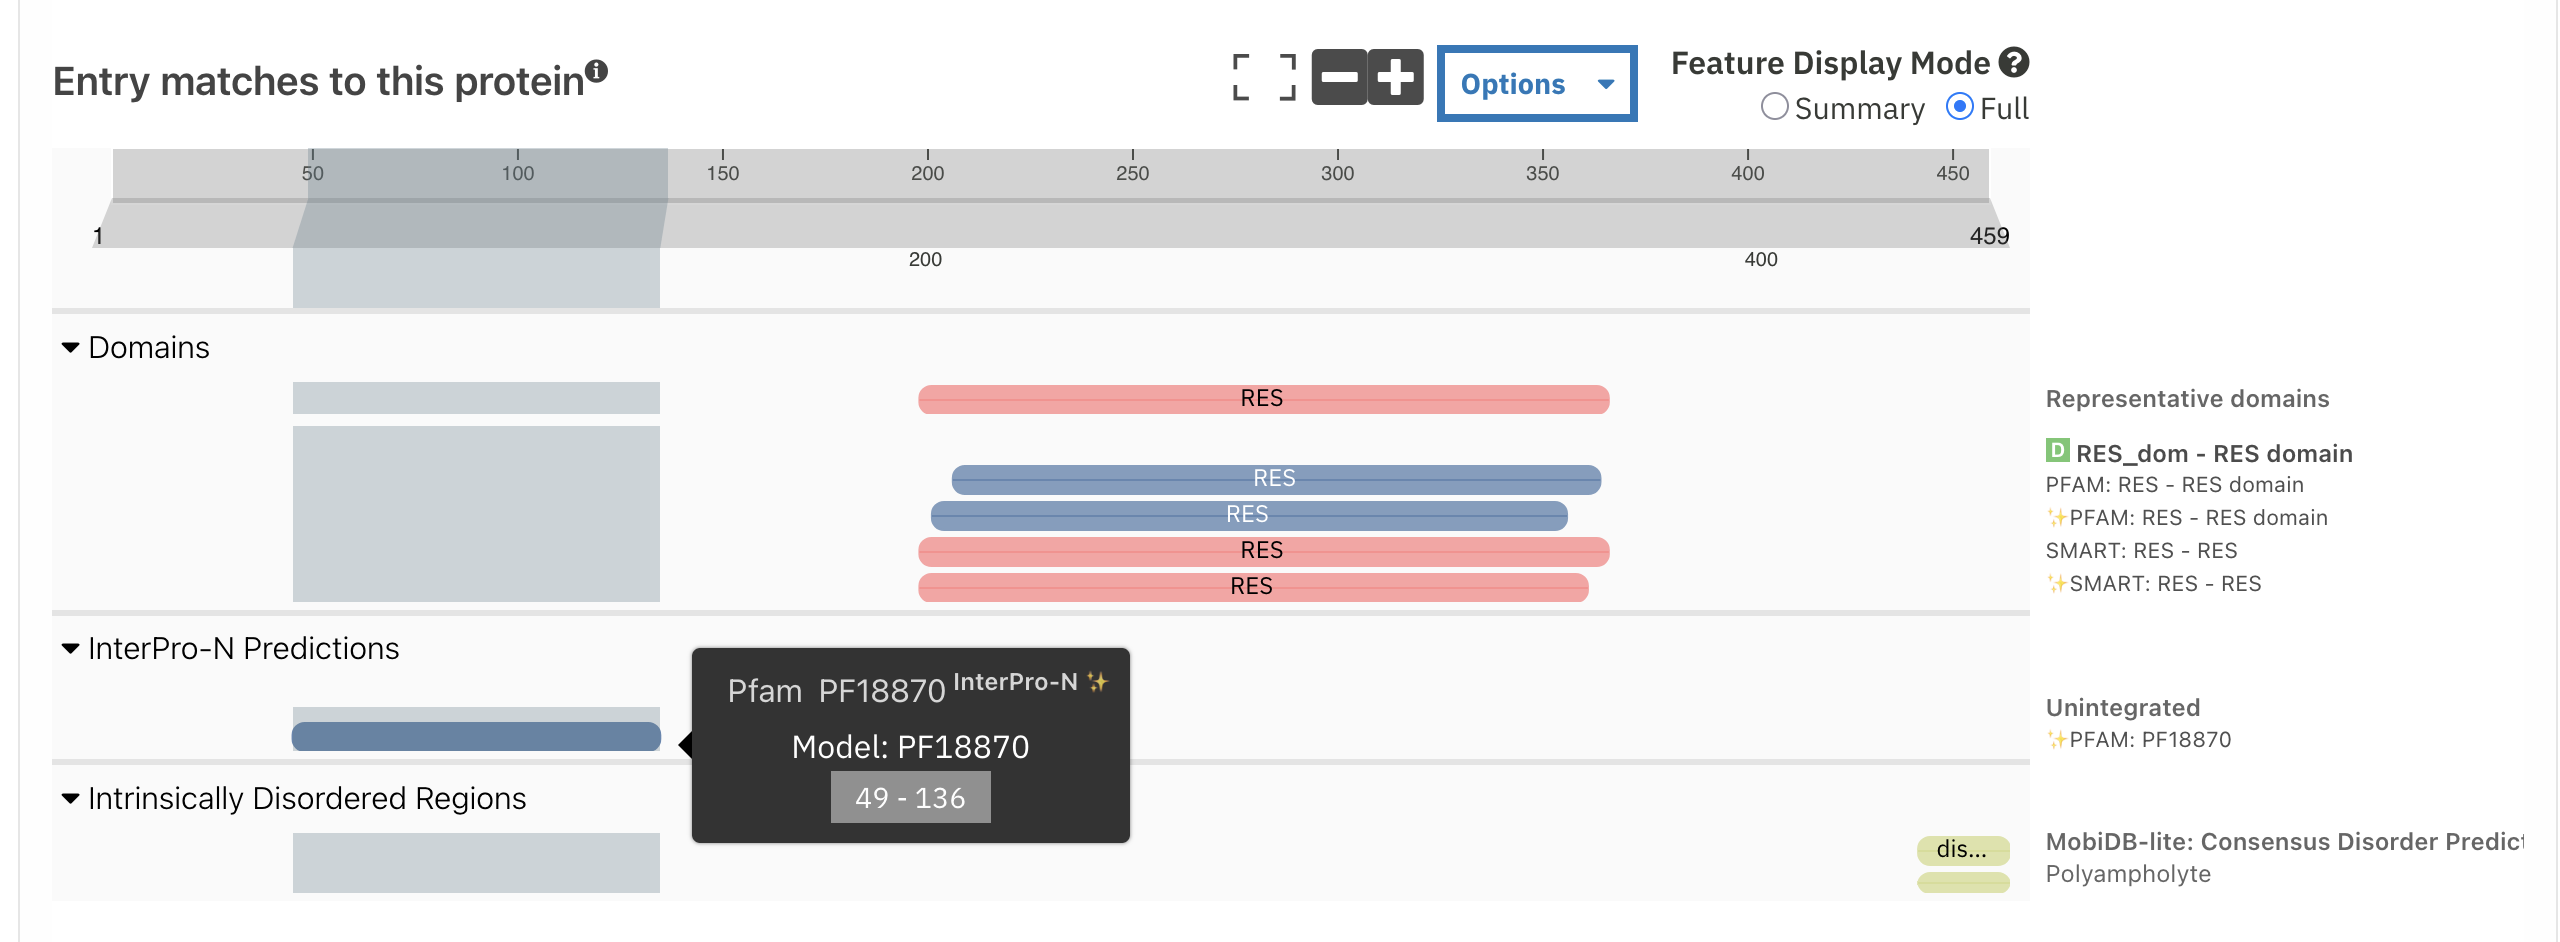
\includegraphics[width=\linewidth]{figs/interpro_domains.png}
\vspace{4pt}

{\footnotesize
\begin{tabular}{@{}llp{3.0cm}@{}}
\toprule
Domain & Range & Note \\
\midrule
PF18870 & 49--136 & no experimental structure exists \\
PF08808 RES & 199--363 & the NADase \\
\bottomrule
\end{tabular}}
\end{minipage}
\hfill
\begin{minipage}[t]{0.49\linewidth}
\vspace{0pt}
\colhead{2.\ Zinc ribbon}
{\footnotesize
\begin{tabular}{@{}ll@{}}
\toprule
Cysteines & \textcolor{zn}{\textbf{C8, C11, C31, C34}} (spacing 3, 20, 3)\\
Pairwise SG--SG (metal-free) & \textbf{3.55--3.81\,\AA}, mean \textbf{3.67\,\AA}\\
Zn--S (metal-bound) & \textbf{2.24--2.25\,\AA}\\
Ideal Zn(Cys)$_4$ edge & \textbf{3.76\,\AA}, deviation \textbf{0.09\,\AA}\\
Mean pLDDT of the 4 Cys & \textbf{90.8}\\
Not disulfides & an S--S bond is 2.05\,\AA\\
Control (T7 gp5) & 10 Cys, \textbf{no cluster}; closest 7.85\,\AA\\
\bottomrule
\end{tabular}}

\vspace{4pt}
\centerline{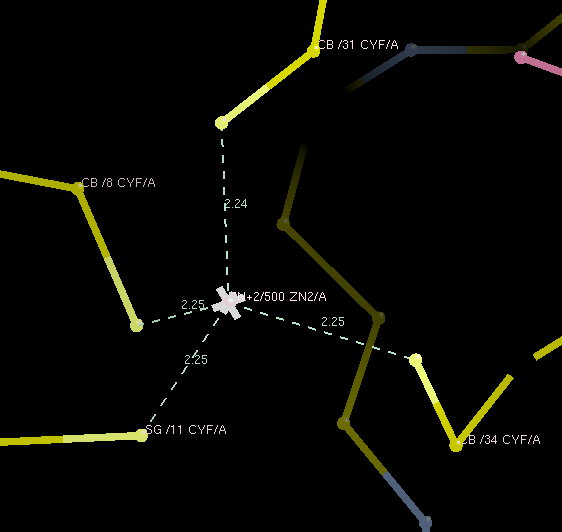
\includegraphics[height=4.6cm]{figs/zn_ribbon.png}}
\vspace{2pt}
{\footnotesize Zn(Cys)$_4$ coordination in the metal-bound model.}
\end{minipage}

\divider

% ===================== ROW 3 =====================
\panelhead{Together they form a bipolar surface}

\begin{minipage}[t]{0.44\linewidth}
\vspace{0pt}
{\small The basic ribbon face and the acidic NTD-1 face sit on adjacent lobes and each faces
solvent. They do not neutralise one another.

\vspace{4pt}
\textbf{Working model (hypothesis).} The N-block recognises a polymerase engaged with nucleic acid:}

{\small
\begin{itemize}[leftmargin=1.2em,itemsep=2pt,topsep=3pt]
  \item the basic zinc ribbon binds the DNA;
  \item the acidic NTD-1 binds the polymerase's basic cleft as a DNA mimic (cf.\ Ocr, T7 gene 0.3).
\end{itemize}}

{\small Consistent with recognition of unrelated polymerases, with $\lambda$ (no phage polymerase),
and with the DNA-free \emph{in vitro} activation.}
\end{minipage}
\hfill
\begin{minipage}[t]{0.53\linewidth}
\vspace{0pt}
\centerline{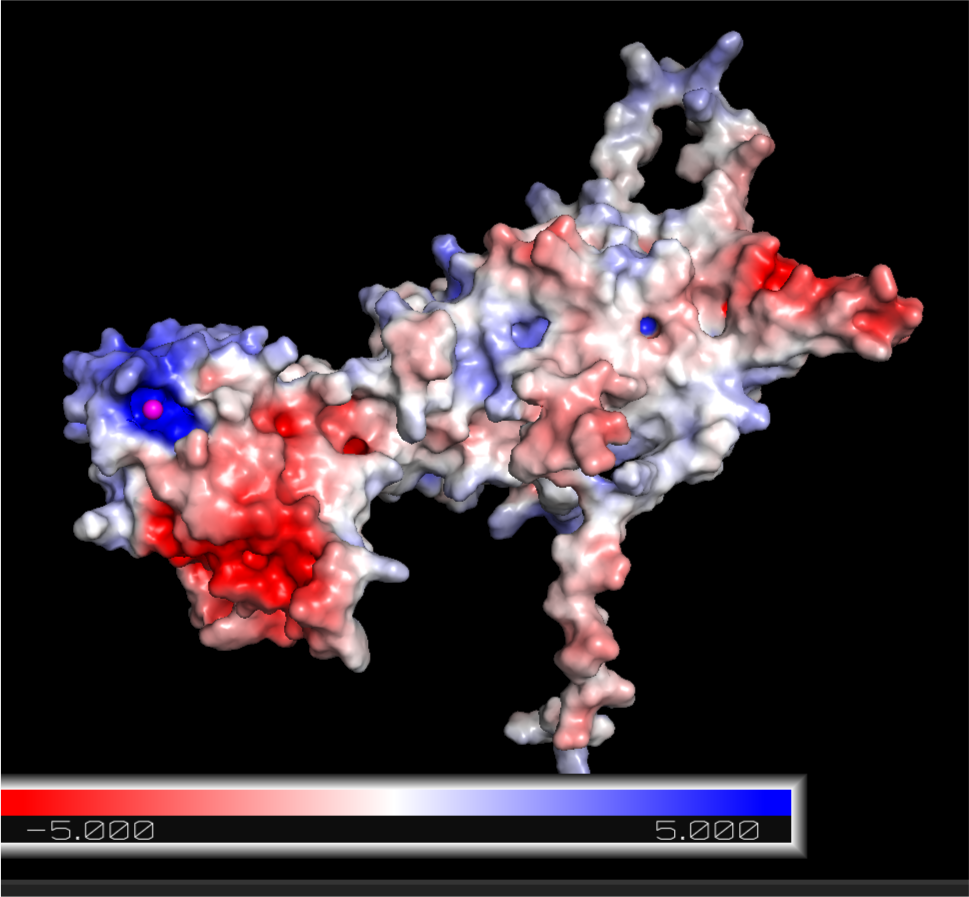
\includegraphics[height=5.6cm]{figs/apbs_surface.png}}
\vspace{2pt}
{\footnotesize Electrostatic surface, $\pm 5\,k_{\mathrm{B}}T/e$.}
\end{minipage}

\vspace{4pt}
{\footnotesize\textcolor{soft}{\textbf{Caveats.} Composition and one predicted model. The rendering
may overstate the basic patch at the zinc if the four Cys were not treated as thiolates. One
orientation. gp5 D106 is itself acidic.
\textbf{Next:} residue-type surface and Zn-deleted control; is D104 on the acidic face; AF3 cofold
with a primer--template duplex; EMSA 1--120 vs 49--136; DNA competition of the aRES--gp5 pull-down.}}

\end{document}
